\chapter{Conclusions}
\label{cha:evaluation}
\section{Summary of Achievements}
In summary, all project aims were fulfilled, except for the cost of service and ease of set-up aims. Other commercially available products cost less, while providing similar or better functions, and the service is very tough to self-deploy.

Core application - OpenFitCompanion was produced, an open-source alternative to health data aggregators and health companions. Providing convenient access to all data in one place with an option to export it to a file, enabling further research such as comparing health tracking devices. Employing nudging mechanisms via daily and weekly reports, where users can effortlessly examine: trends and progress towards their goals. Leveraging AI to create activity plans, curating exercises to align with user's preferences and needs, with exercise reminders sent via push-notifications. Lastly, enabling a natural language conversation about user's health data, mimicking interaction with a personal trainer at a fraction of the cost. System structure was explained with the help of diagrams and key decisions justified. If AI is not used, the application is a strong alternative to similar systems like Google Fit. Although, AI functions within the application can provide useful insights, it also raises the operating cost to where it is hard to justify that our product is a better alternative. 

Data analysis was performed in order to answer research question concerning the equivalence of used devices. Finding of exploration were presented: Bland-Altman plots, implications of initial findings and outlier protocol. Empirical difference percentages were calculated. Hypothesis testing problem was formulated, with the justification of statistical test used. Finally, results were interpreted showing evidence of significant difference in measurement of different activity intensity seconds. Still, it is merely an interesting observation that warrants conducting a more formal, rigorous study involving more participants and stricter data gathering methodology. The artefact could enable such studies to be performed in a cost-effective and transparent manner.
\section{Critical Reflection}
\subsection{Product \& Investigation}
Cost was one of the driving factors to develop OpenFitCompanion, so that users can enjoy features that commercial products lock behind a an expensive subscription. Although there is one product that OpenFitCompanion beats on cost, it loses to all others. Another model or approach should have been tried. 

Open-source was also a key point, however, a lot of closed source and non portable technologies have been used. Deploying on closed-source cloud like AWS and storing data in DynamoDB restrict options for further extension and possible migration. More open technologies should have been used to stay true to the product's name - OpenFitCompanion.

The project is not very attractive to potential open-source contributors due to absence of tests and a very manual deployment procedure. Tests allow collaborators to feel confident about system changes, ensuring no functional regression takes place. At least for very critical portions, tests should have been created. Regarding deployment process, the project requires zipping lambda function folders and uploading them on the AWS web console one by one after every change. For a project that is cloud-centric, more attention should have been dedicated to automating deployment pipeline.

User errors definitely took place during data collection for the analysis. They could caused differences between devices that were not detected via used outlier detection protocol. A more rigorous methodology for data collection should have been, such as journaling each day to sanity-check measurements from each device. 
\subsection{Personal}
I think the biggest difficulty was my lack of planning. As this project was self-proposed, I was in charge of coming up with requirements. Initially coming up with a very simplistic system that would not have enough complexity. My philosophy was to first finish that and if I have time then expand to more features. After finishing that simple application, with the help of my supervisor and wearables lab I got very interesting feature ideas  such as incorporating a second device and using LLMs. However, the foundation of the system was too simple and could not those features, so I have re-structured the system many times. I think I wasted a good chunk of time doing that, whereas I should have spent more time planning before implementation. Alternatively, I could have employed agile methodology and developed the system with high degrees of modularity and flexibility, therefore being able to cope with changing requirements more easily.

The previous point also lead to me not having a clear schedule, mostly bouncing between working on different features with no deadlines set. Especially with LLM integration, I spent too much time on designing prompts, trying to improve reliability, etc. This led me to have less time to polish other implementation aspects as well as working on the screencast and this report. I also tunnel-visioned on trying to make GPT4 work, whereas trying different models might have been more beneficial. 
\section{Further Work}
\subsection{Reducing AI inference cost}
\label{subsec:tryingOther}
As discussed in evaluation \ref{cha:evaluation}, the service does not compare well to other products mainly due to cost of using GPT4 with Knowledge Retrieval (RAG), which is still an experimental feature at the time of writing. Maybe OpenAI improves the feature and allows more tuning, however as it currently stands other models should be examined. An obvious choice would be open-source models like LLAMA-2 or recently released Grok-1, as on the surface they are free to use. However, they are hard to set up and require commercial level ML machines with a lot of VRAM, this is the reason they were not used initially. Cloud deployment is a more realistic prospect, with a rough estimate of using AWS Sagemaker to run LLAMA-2-13B on demand costing 7£ per month. Still, open-source models perform worse than commercial ones like GPT4, whether utility is preserved while reducing costs remains to be seen via experimentation.

The other option is to use newer commercial model. For example Claude 3 Sonnet, performs almost equally with GPT4, and even surpassing it, at a fraction of the cost. It is hard to classify which LLM benchmark reflects the nature of the task at hand, so the safe option is "Mixed evaluations (BIG-Bench-Hard)" benchmark, which contains a mix of different tasks, serving as a kind of an IQ test for LLMs. Sonnet has 82.9\% performance against 83.1\% of GPT4 \cite{claude3Bench}, while having a cost of 3\$ per 1M tokens, which is 333\% less than GPT4.

\subsection{Utilizing LLM vision}
First idea is to use visual modality in LLMs for nutrition management. Nutrition is as important as exercise or sleep for improving overall health. Existing commercial products mostly involve manually putting ingredients and it's quantity to estimate calories and macro-nutrients from the meal. However, this feature would involve just taking a picture of the meal, which is then processed by an LLM. MyfitnessPal has similar feature where you scan the meal using the camera; however, from the demo and user feedback, it is apparent that it requires having very cleanly separated ingredients which are scanned from different zoom levels separately, struggling with meals where ingredients are slightly mixed. Preliminary investigation using Claude 3 Sonnet shows promise, it guesses ingredients of a dish \ref{fig:sonnetV1} somewhat correctly, and then approximates the weight of each one \ref{fig:sonnetV2}.

Second idea is to force users to go to the gym by requiring taking a selfie in the gym on designated days. This would probably go beyond nudging and be considered an intervention. However, feeling that something is keeping you accountable can be encouraging as well. The process would involve taking a fresh picture of the user with some distinct gym equipment in the background, then using LLM to verify if its the same user and that they are in the gym. Camera API would be used rather than image upload, as users may upload old photos. Personalised encouraging messages could be sent on failure to verify, such as how many MET minutes the gym workout would contribute to reaching the weekly goal. 
\begin{figure}
    
    \centering
    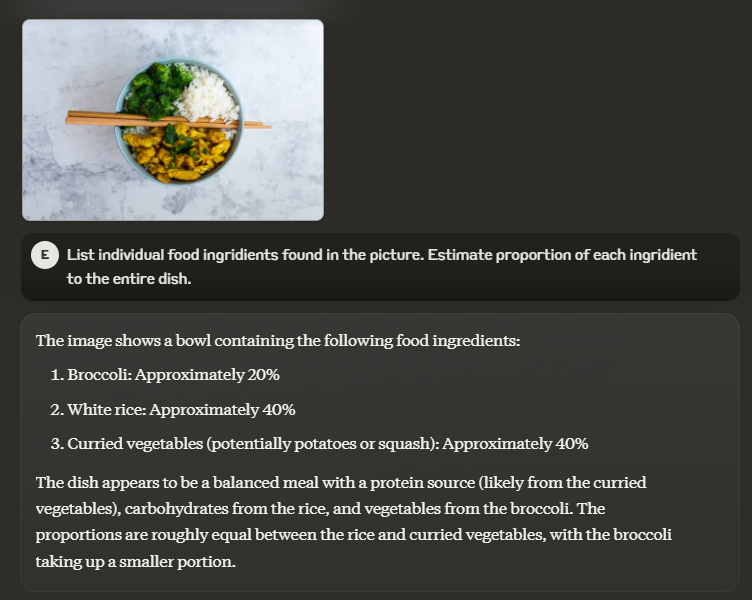
\includegraphics[width=1\textwidth,keepaspectratio]{../images/sonnet_vision.png}
    \caption{Claude 3 Sonnet identifies ingredients in a dish}
    \label{fig:sonnetV1}
    
\end{figure}
\begin{figure}
    
    \centering
    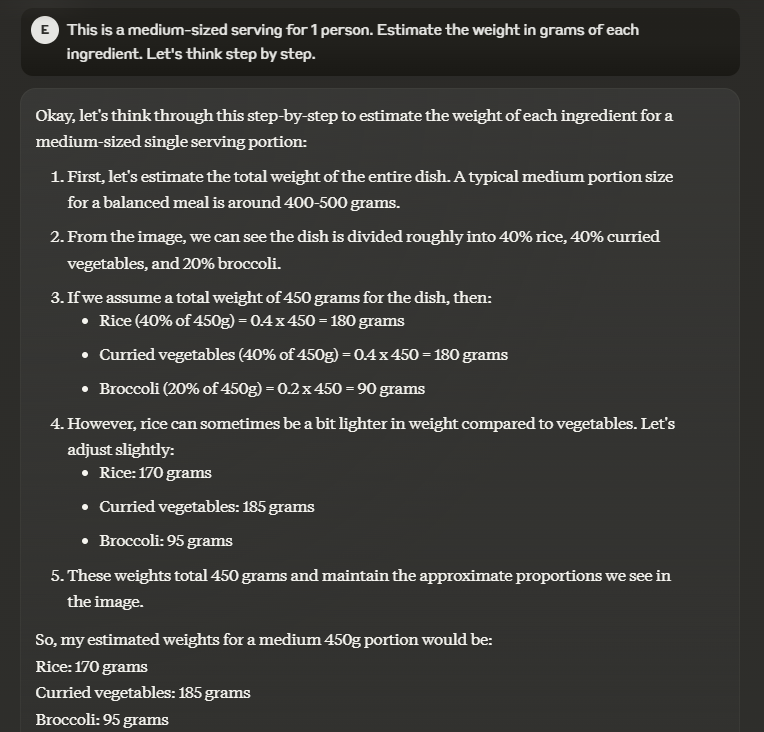
\includegraphics[width=1\textwidth,keepaspectratio]{../images/sonnet_vision_2.png}
    \caption{Claude 3 Sonnet approximates weight of each ingredient of a dish}
    \label{fig:sonnetV2}
    
\end{figure}

\subsection{Avoiding Cloud vendor lock-in}
Cloud providers like AWS try to make it hard to switch to another provider. For example, Lambda's data out is free of charge as long as the destination is another AWS service. AWS were to raise prices, it would be a laborious task to replicate the functionality on another cloud, like Azure. Then Azure could raise prices as well, requiring another rewrite or just accepting the situation and overpaying. 

One option is OpenStack. It is a fundamentally different approach - it is an open-source, private cloud solution. Whereby you have similar components of a typical cloud infrastructure but deployed on particular machine. OpenStack is software which can run on any linux machine, so it can be deployed on either a physical machine or a VM. Physical machine would involve maintenance, which would be unreasonable for most users. Deploying on a VM, like AWS EC2 instance would be more practical as it won't require physical maintenance. However, it would still involve a complex set-up. Taking this option woul make the project cloud provider independent, able to deploy on physical machines or on any VM from any provider. Notably, Mixtral provides ready to deploy OpenStack system to self-deploy their LLM, so this could tie with earlier suggestion \ref{subsec:tryingOther} of trying other LLM models 

Terraform is another option. It is an Infrastructure as Code (IAC) solution, allowing writing infrastructure using textual configuration files. CloudFormation is used within this project, but it only supports AWS only, whereas Terraform is cross-platform and supports all major cloud providers. It would not prevent lock-in like OpenStack would, but it would make it easier to migrate or use multi-cloud strategy. It would also improve existing self-deployment process, as it could automatically fill in template fields such as secret keys from a configuration file, whereas currently the user has to use web console and complete the process of filling variables manually.

